 \documentclass[book.tex]{subfiles}
\begin{document}

\section{Action Phase: Adaptive Tile Refreshment}
After the player is done setting up the game, it is time for the scrolling engine to shine. On bitmapped displays without hardware scrolling like the EGA card, the entire screen have to be erased and redrawn in the slightly shifted position whenever the player moved in any direction. This would kill the CPU as you need to update all pixels of all four planes on the EGA card (remember the planar mapping of chapter \#\#\#?).\\ 

So here John Carmack came with a smart solution. The scrolling engine is based on a simple yet powerful technology called Adaptive Tile Refreshment. The core idea is to  refresh only those tiles on the screen that needed to change.\\

The visible screen is divided into tiles of 16x16 pixels. On a screen with 320x200 pixels, it means a grid of 20x13 tiles (actually it is 12.5 tiles high, but we need to round to integer). Let's look at \textit{Commander Keen 1: Marooned on Mars} in Figure \ref{fig:keen_difference}. This is the first level of Marooned, immediately to the right of the crashed Bean-with-Bacon Megarocket. The first figure is the start of the level, the second figure is after Keen has moved one tile (16 pixels) to the right through the world. They look almost identical to the naked eye, don't they? \\

Now, if we perform a difference on both images you see which tiles needs to be changed upon screen refresh. The trick behind the scrolling in the first Commander Keen games was to only redraw tiles that actually changed after panning 16 pixels (one tile), since most maps had large swathes of constant background. In case of Figure \ref{fig:keen_difference} only 69 tiles of the total 260 tiles need to be refreshed, which is 27\% of the screen! 


\pagebreak
\begin{figure}[H] 
  \centering 
  \frame{\scaledimage{0.6}{game/keen-screen1.png} }
\end{figure}
\begin{figure}[H] 
  \centering 
  \frame{\scaledimage{0.6}{game/keen-screen2.png} }
\end{figure}
\begin{figure}[H] 
  \centering 
  \frame{\scaledimage{0.6}{game/keen-difference.png} }
  \caption{Start of the world, moved one tile to the right and difference.}
  \label{fig:keen_difference}
\end{figure}
\pagebreak

So everytime Keen is crossing one tile the entire level is 'jolted' 16 pixels. This 'jolted' doesn't feel like a smooth scrolling game. Luckily, the EGA card provides two hardware features that support smooth pixel scrolling: setting the CRTC Start Address and Horizontal PEL Panning Registers. \\

\subsection{EGA Virtual Screen}

The EGA adds a powerful twist to linear addressing: the logical width of the virtual screen in VRAM memory need not to be the same as the physical width of the screen display. The programmer is free to define a logical screen width of up to 4096 pixels and then use the physical screen as a window onto any part of the virtual screen. What's more, a virtual screen can have any logical height up to the capacity of the VRAM memory. The logical width of the virtual screen is expressed in the number of words of display memory considered to make up one scan line. So 20 words of display memory is setting a scan line of 320 pixels. The code below illustrates how to change the logical width.\\

\begin{minipage}{\textwidth}
  \lstinputlisting[language=C]{code/SCREEN_WIDTH.ASM}
  \end{minipage}
  \label{ega_pel_pan}
  \par

The area of the virtual screen displayed at any given time is selected by setting the display memory address at which to begin fetching video data. This is set by way of the Start Address register. The default address is \cw{A000:0000h}, but the offset can be changed to any other number. In EGA's planar graphics modes, the eight bits in each byte of video RAM correspond to eight consecutive pixels on-screen. Panning down a scan line requires only that the start address is increased by the logical width in bytes. Horizontal panning is possible by increasing the start address by one byte, although in this case only relative coarse of 8 pixels (1 byte)  adjustments are supported. See the code below how to set the Start Address register.

\begin{minipage}{\textwidth}
  \lstinputlisting[language=C]{code/EGA_SET_ADDRESS.ASM}
  \end{minipage}
  \label{ega_set_address}
  \par

\subsection{Horizontal Pel Panning}
Smooth pixel scrolling of the screen is provided by the Horizontal Pel Panning register in the Attribute Controller (ATC). Up to 7 pixels' worth of single pixel panning of the displayed image to the left is performed by increasing the register from 0 to 7. This exhaust the range of motion possible via the Horizontal Pel Panning register. The next pixel's worth of smooth panning is accomplished by incrementing the Start Address register by one byte and resetting the Horizontal Pel Panning register to 0. \\

Horizontal PEL Panning Registers will resolve the final 8 pixels 'jolt'. By setting the first 4 bits of the register we select the number of pixels to shift the entire screen up to 8 pixels horizontally to the left. As long as Keen is within the 16 pixels of a tile, scrolling is supported by EGA hardware and the game doesn't need to use any CPU time to scroll the screen.\\

There is one annoying quirk about programming the Attribute Controller: when the ATC Index register is set, only the lower five bits (bits 0-4) are used as the internal index. The next most significant bit, bit 5, controls the source of the video data send to the monitor by the EGA card. When bit 5 is set to 1, the ouput of the palette RAM controls the displayed pixels; this is normal operation. When bit 5 is 0, video data doesn't come from the palette RAM, and the screen becomes a solid color. To ensure the ATC index register is restored to normal video, we must set bit 5 to 1 by writing \cw{20h} to the register.\\ 

\begin{minipage}{\textwidth}
  \lstinputlisting[language=C]{code/EGA_PELPAN.ASM}
  \end{minipage}
  \label{ega_pel_pan}
  \par

So the smooth horizontal and vertical panning should be viewed as a series 16-pixel tile refreshment and fine adjustments in the 8-pixel range between coarse byte-sized adjustments as illustrated in Figure \ref{fig:tile_refresh} 

\begin{figure}[H]
\centering
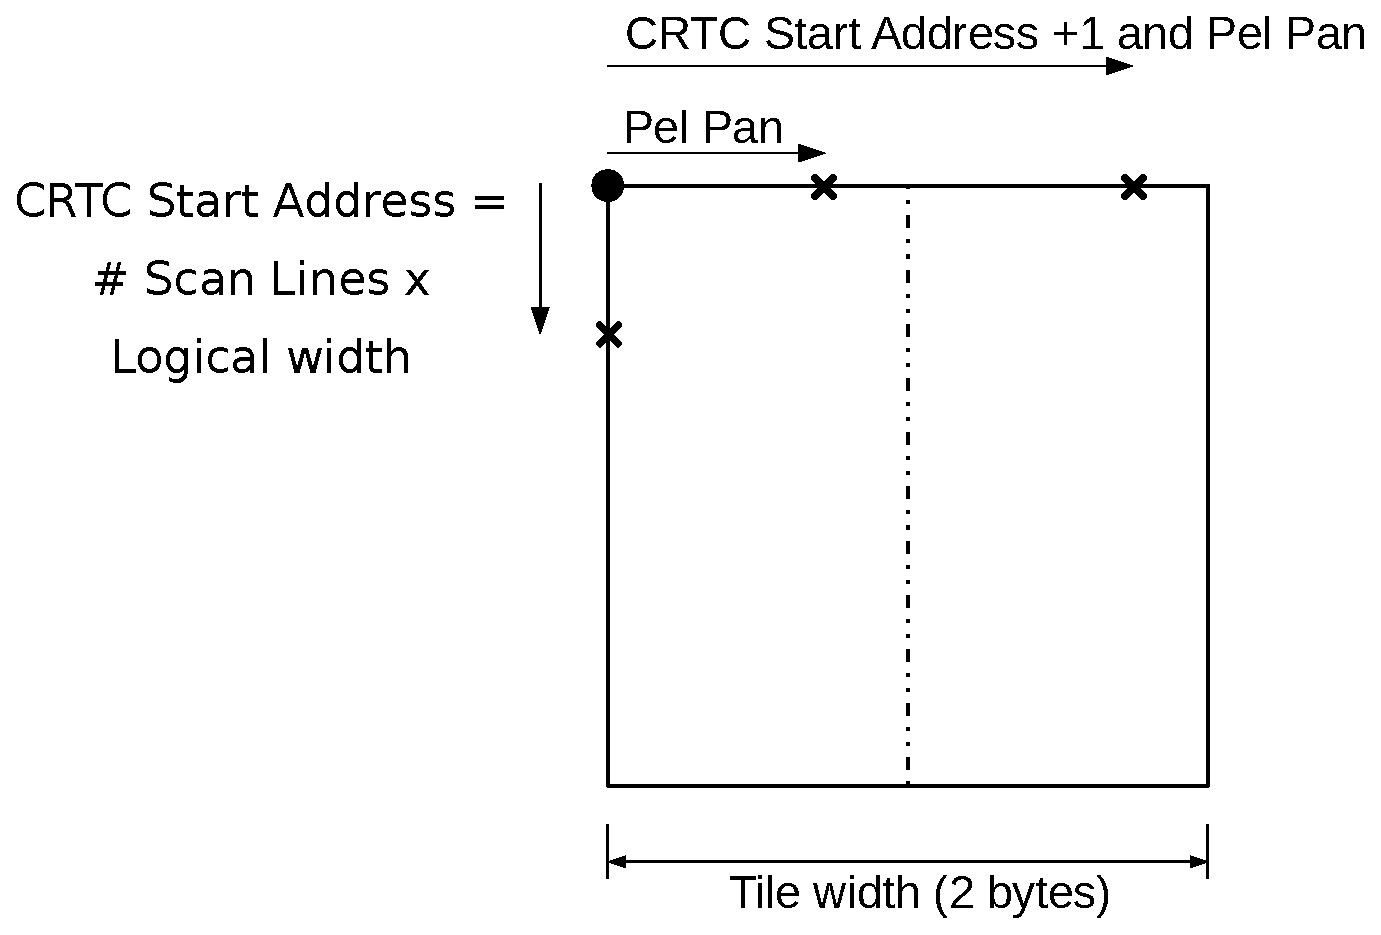
\includegraphics[width=\textwidth]{imgs/drawings/Tile_Refresh.eps}
\caption{Smooth scrolling in EGA.}
\label{fig:tile_refresh}
\end{figure}

\begin{minipage}{\textwidth}
  \lstinputlisting[language=C]{code/EGA_REFRESH.ASM}
  \end{minipage}
  \label{ega_refresh}
  \par





\section{View Port and Buffer setup}
First we need to explain how the view port and buffer layout are setup. The visible viewing screen has a resolution of 320x200 pixels. If we translate this into 16x16 pixel tiles, we have a screen view size of 20x13 tiles. By making the view port one tile higher and wider than the screen (21x14 tiles), we can scroll the screen up to 16 pixels without any tile refresh to the right or bottom side of the screen using the Start Address and Pel Pan registers. Finally, we create an update buffer that has enough space to float the view port up to two tiles in all direction.\\

So summarized, as can be seen in Figure \ref{fig:screen_setup}, the following tile views are defined:
\begin{itemize}
\item Screen View size of 20x13 tiles and Port View size of 21x14 tiles.
\item Buffer screen size of 22x14 tiles. This is one tile wider than the Port View, where the additional tile is used to mark a '0' at the end of each tile row. Notice that in the code the UPDATESCREENSIZE value is defined as (UPDATEWIDE * UPDATEHEIGHT + 2). The additional 2 bytes are used to store a termination indicator at the very end of the buffer screen.
\item Total buffer size is stored in UPDATESIZE, which contains the UPDATESCREENSIZE and 2 two times a spare buffer to support the floating of two tiles in any direction. 
\end{itemize}
\par
 
\begin{figure}[H]
\centering
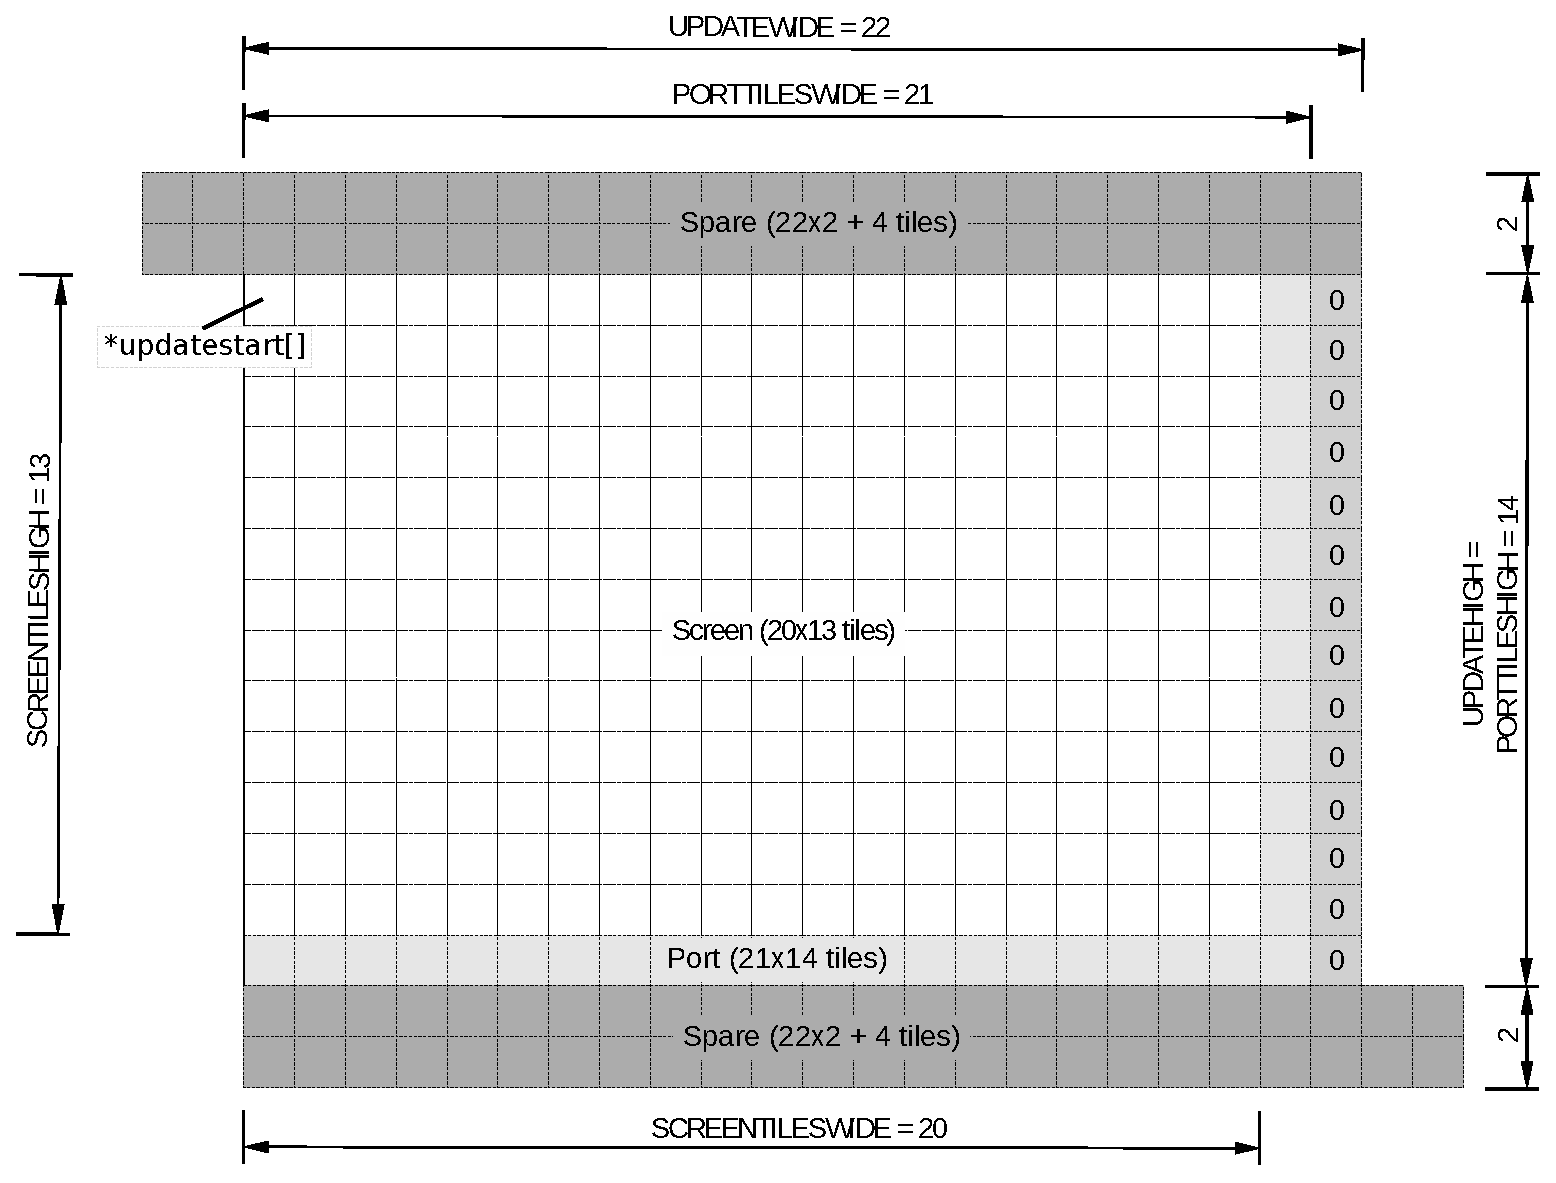
\includegraphics[width=\textwidth]{imgs/drawings/buffer_tile_layout.eps}
\caption{View and buffer port layout.}
\label{fig:screen_setup}
\end{figure}



\section{Screen buffer}
Even if the screen is not scrolling, tile refreshes are required to support sprite animations. Since moving a sprite in this way involves first erasing it and then redrawing it, the image of the erased sprite may be visible briefly, causing flicker. This is where double buffering comes in: setting up a second buffer into which the code can draw while the first buffer is being shown on screen, which is then switched out during screen refresh. This ensures that no frame is ever displayed mid-drawing, which yields smooth, flicker-free animation.\\

Now, let's have a closer look at the EGA memory setup. As explained in the previous section, the view port has a size of 21x14 tiles, which is 336x224 pixels. That means the logical width in VRAM must be at least 336 pixels (42 bytes) wide. In the file \cw{id\_vw.h} the VRAM screen buffer is defined by SCREENSPACE, which is set to 64x240 bytes, or 512x240 pixels. This is more than sufficient to update one virtual screen in VRAM.\\

Since one screen only used 15,360 bytes of VRAM (which is 3,840 bytes per plane), we have more than enough space to store more than two full screens of video data. The video memory is organized into three virtual screens:
\begin{itemize}
\item Page 0 and 1, which are used to switch between buffer and view screen
\item A master page containing all tiles and sprites, which are copied to the buffer memory when performing the screen update.
\end{itemize}
\par

\begin{figure}[H]
\centering
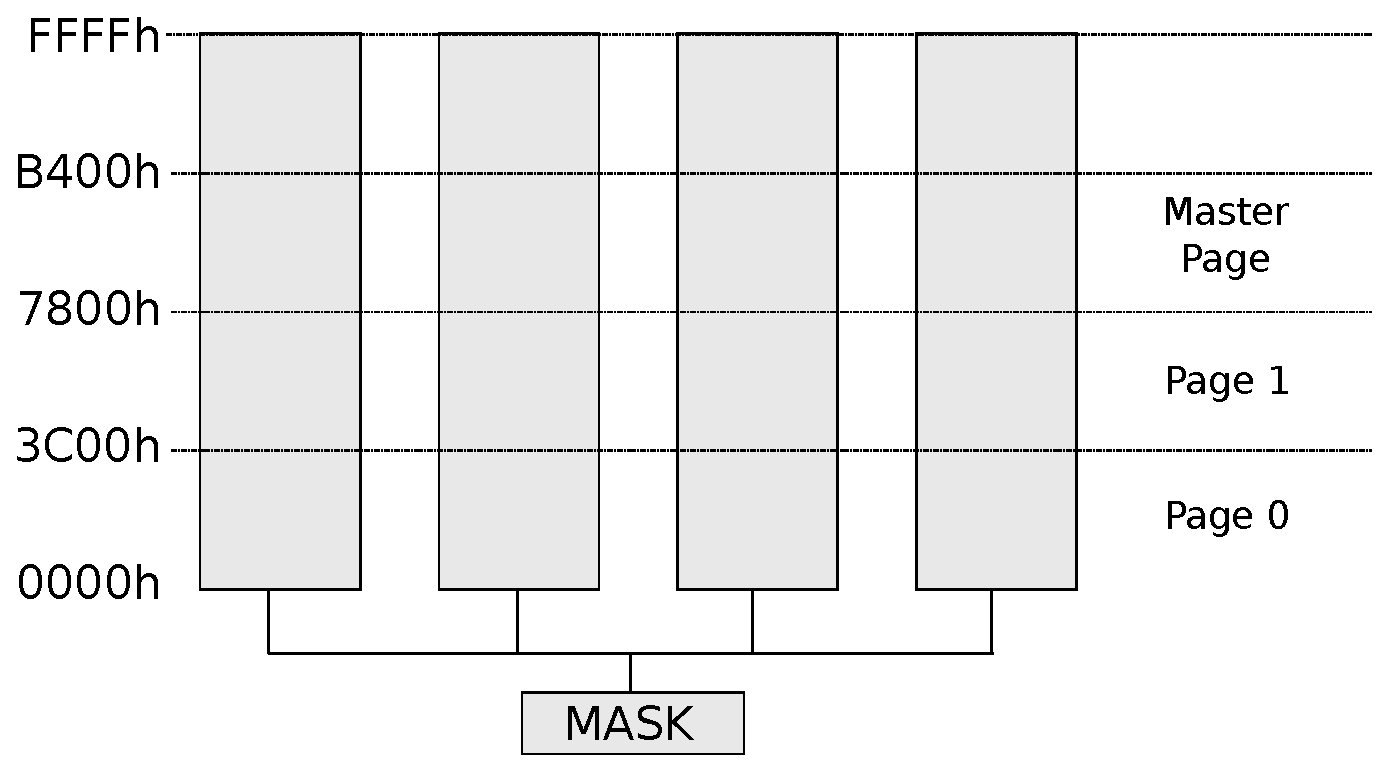
\includegraphics[width=\textwidth]{imgs/drawings/ega_ram_architecture.eps}
\label{fig:ega_ram_arch}
\end{figure}

The page that is actually displayed at any given time is selected by setting the Start Address register at which to begin fetching video data.\\

\section{Global coordinate system}
The game and all actors are defined in a global coordinate system, which is scaled to 16 times a pixel. The higher resolution enables more precision of movements and better simulation of movement acceleration. Conversion between global, pixel and tile coordinate systems can be easily performed by bit shift operations:
\begin{itemize}
\item From global to pixel is shifing 4 bits to right.
\item From pixel to tile is shifting 4 bits to right.
\item From global to tile is shifting 8 bits to right.
\end{itemize}

The idea is to first perform all actions and movements in the global coordinate system, and then move back to pixels or tile coordinate system for video updates.



\section{Life of a 2D Frame}
The approach of refreshing the screen is different between the first Commander Keen games, Commander Keen 1-3, and the ones after. In the first games the algoritm keeps the screen view and buffer at fixed VRAM locations, where it performs a check which tiles are changed after the scroll. In the later games, it makes use of the moving the VRAM location and add a full row or column at the beginning or end of the view port. 
\\
\subsection{Screen refresh in Commander Keen 1-3}
In the this section we explain how the first games are working\footnote{We can only explain how the algoritm is working without code examples, since the only released code is Keen Dreams which is using the improved algoritm.}. Six stages are involved in drawing a 2D scene:
\begin{enumerate}
\item Check if the player has moved one tile in any direction.
\item Validate which tiles have changed (both from scrolling and animated tiles), copy these respective tiles to the Master view in VRAM and mark the tiles to be updated in the next refresh in both the screenpage and otherpage update list.
\item Refresh the buffer view by scanning all tiles. If a tile needs to be updated, copy the tile from the master view to the buffer view in VRAM.
\item Iterate through the removal list and copy corresponding image block from master view to buffer view in VRAM. 
\item Iterate through the sprite list and copy corresponding sprite image block from asset location in RAM to buffer view in VRAM
\item Switch the screen and buffer view by adjusting the Start Address and Pel Panning registers.
\end{enumerate}

In the next six screenshots, we take you step-by-step to each of the stages. The screen has to scroll one tile to the right.

\begin{figure}[H]
\centering
 \fullimage{/game/Scroll_KC1-3_1.png}
 \caption{Step 1: Player moved to the right and forces the screen to scroll}
 \label{fig:kc1_3_start}
\end{figure}

\begin{figure}[H]
\centering
 \fullimage{/game/Scroll_KC1-3_1-scroll_master.png}
 \caption{Step 2: Update changed tiles in masterscreen}
 \label{fig:kc1_3_update_masterscreen}
\end{figure}


\begin{minipage}{.4\textwidth}
Each tile of the buffer screen is compared with the tile on the corresponding level location. If the tile number has changed, the tile is updated by copying tile data from the asset location into the corresponding location in the VRAM of the masterscreen.\\
\par
In parallel each tile in both visible and buffer tile array will be marked with a '1', which means it needs to be updated on the next refresh.
 \end{minipage}
\begin{minipage}{.6\textwidth}
\begin{figure}[H]
  \centering
 
\includegraphics[width=.9\textwidth]{screenshots_300dpi/game/Scroll_KC1-3_1-scroll_update.png}
 \label{fig:kc1_3_update_refresh_img_1}  
\end{figure}
\end{minipage}

\pagebreak

\begin{figure}[H]
\centering
 \fullimage{/game/Scroll_KC1-3_1_remove.png}
 \caption{Step 3 and 4: Copy changed tiles and removed sprites from Master screen to buffer screen}
 \label{fig:kc1_3_update_remove}
\end{figure}


\begin{minipage}{.4\textwidth}
Scan all tiles in the buffer tile array and for each tile marked as '1', copy the tile from master to buffer screen in VRAM.\\
\par
If a sprite has moved, the previous sprite location is added to the block removal list. For each block in this list, copy the width and height size of the sprite block (marked in orange in Figure \ref{fig:kc1_3_update_remove}) and mark the corresponding tiles in the buffer tile array with a '2'.
 \end{minipage}
\begin{minipage}{.6\textwidth}
\begin{figure}[H]
  \centering
 
\includegraphics[width=.9\textwidth]{screenshots_300dpi/game/Scroll_KC1-3_1-update_remove.png}
 \label{fig:kc1_3_update_remove_img_1}  
\end{figure}
\end{minipage}

\pagebreak

\begin{figure}[H]
\centering
 \fullimage{/game/Scroll_KC1-3_1_sprite.png}
 \caption{Step 5: Scan sprite list and copy sprite onto buffer screen}
 \label{fig:kc1_3_update_sprite}
\end{figure}


\begin{minipage}{.4\textwidth}
Scan the sprite list. Validate if the sprite is in the visible part of the view port and copy the sprite image into the VRAM buffer screen. Mark the corresponding tiles in the buffer tile array with a '3'.
 \end{minipage}
\begin{minipage}{.6\textwidth}
\begin{figure}[H]
  \centering
 
\includegraphics[width=.9\textwidth]{screenshots_300dpi/game/Scroll_KC1-3_1-update_sprite.png}
 \label{fig:kc1_3_update_sprite_img_1}  
\end{figure}
\end{minipage}

\pagebreak

\begin{figure}[H]
\centering
 \fullimage{/game/Scroll_KC1-3_1_final.png}
 \caption{Step 6: Swap buffer and screen page}
 \label{fig:kc1_3_update_final}
\end{figure}


\begin{minipage}{.4\textwidth}
Swap the buffer and screen page by updating the CRTR start address and horizontal Pel Panning. The buffer tile array is cleared to '0', and then buffer and visible tile arrays are swapped. Then step 1 is repeated. 
 \end{minipage}
\begin{minipage}{.6\textwidth}
\begin{figure}[H]
  \centering
 
\includegraphics[width=.9\textwidth]{screenshots_300dpi/game/Scroll_KC1-3_1-scroll_final.png}
 \label{fig:kc1_3_update_final_img_1}  
\end{figure}
\end{minipage}


\pagebreak

Note that step 2 and 3 (except for the animated tiles) only needs to happen if Commander Keen is moving more than 16 pixels, where step 4 and 5 normally needs to happen for each refresh.
So the number of drawing operations required during each refresh is controllable by the level designer. If they choose to place large regions of identical tiles (the large swathes of constant background), less redrawing (meaning: less redrawing in step 2 and 3) is required.

\subsection{Screen refresh in Commander Keen 4-6}
In the later versions of Commander Keen, John Carmack explored what would happen if you push the virtual screen over de 64K, or \cw{0xFFFF}, border in video memory. It turned out that the EGA continues the virtual screen at \cw{0x0000}. This means you could wrap the virtual screen around  the EGA memory and only need to add a stroke of tiles on one of the edges when Commander Keen moved more than 16 pixels.
\\
\begin{figure}[H]
  \centering
  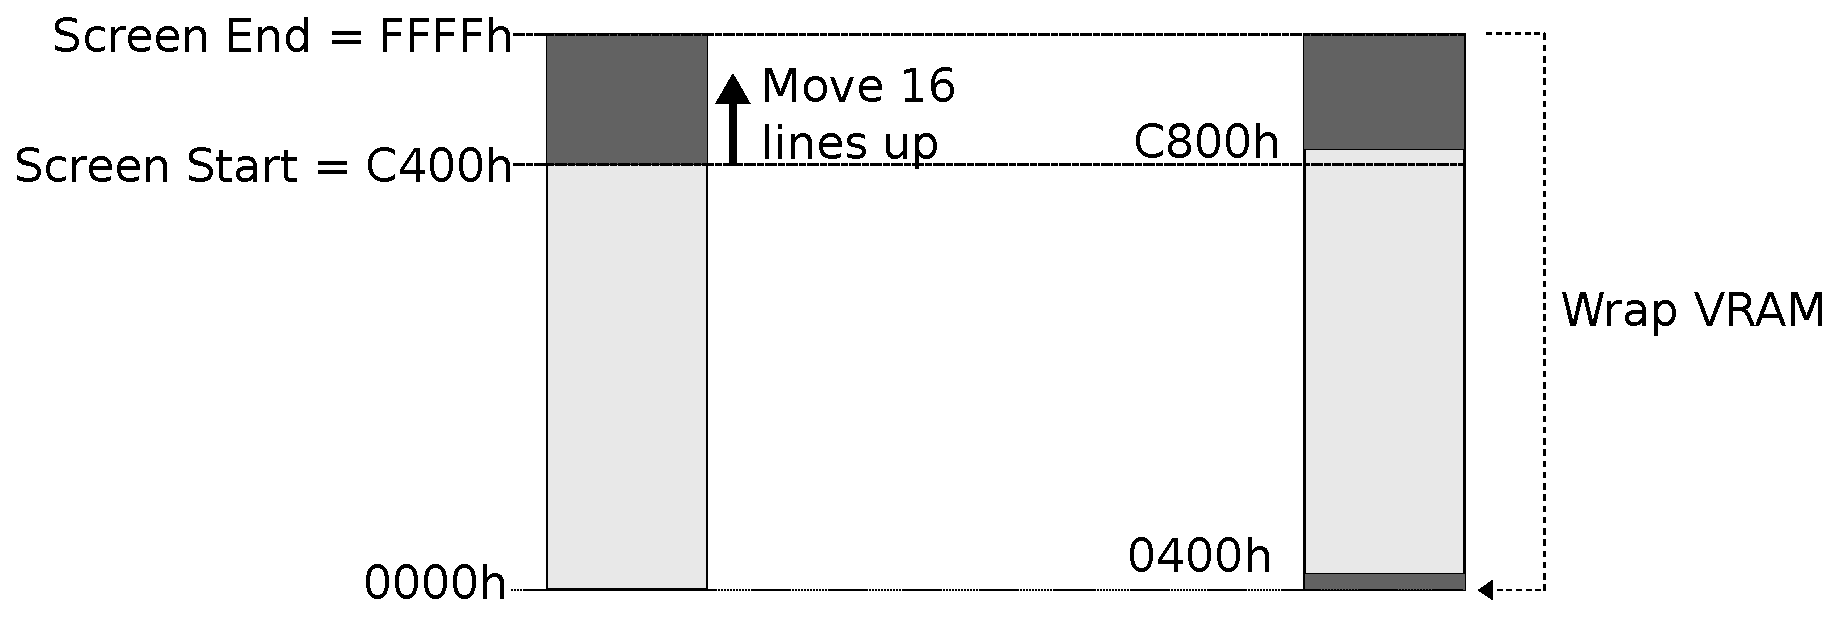
\includegraphics[width=\textwidth]{imgs/drawings/ega_wrapping.eps}
  \label{fig:ega_wrapping}
  \caption{Wrap virtual screen around the EGA memory}
\end{figure}

This results in the following algoritm to scroll and refresh the screen:
\begin{enumerate}
\item Check if the player has moved one tile in any direction.
\item In case the player moved one tile, add the respective column or row in the Master view in VRAM and flag the new tiles of column/row to be updated in the next refresh for both the screenpage and otherpage update list. Update the screenstart and buffer tile array pointers as well.
\item Refresh the buffer view by scanning all tiles. If a tile needs to be updated, copy the tile from the master view to the buffer view in VRAM.
\item Remove the opposite row/column from the Master view.
\item Iterate through the removal list and copy corresponding image block from master view to buffer view in VRAM. 
\item Iterate through the sprite list and copy corresponding sprite image block from asset location in RAM to buffer view in VRAM
\item Switch the screen and buffer view by adjusting the Start Address and Pel Panning registers.
\end{enumerate}


In the next screenshots we explain only steps that are different compared to Commander Keen 1-3 as explained before.
\\

\begin{figure}[H]
\centering
 \fullimage{/game/Scroll_KC4_6_1.png}
 \caption{Step 1: Player moved to the left and forces the screen to scroll}
 \label{fig:kc4_6_start}
\end{figure}

\begin{figure}[H]
\centering
 \fullimage{/game/Scroll_KC4_6_2.png}
 \caption{Step 2: Move screen start and add column to VRAM}
 \label{fig:kc4_6_add_column}
\end{figure}


\begin{minipage}{.4\textwidth}
Decrease the screenstart of all three screen locations 2 bytes (1 tile). Copy a left-column of tiles from the asset location into the corresponding location in the VRAM of the masterscreen.\\
\par
In parallel decrease both tile array pointers one byte and mark each tile on the left border in both the visible and buffer tile array with '1', so it is updated upon the next refresh.
Finally, the most right column (which is now outside the view port) is marked with a '0'.
 \end{minipage}
\begin{minipage}{.6\textwidth}
\begin{figure}[H]
  \centering
 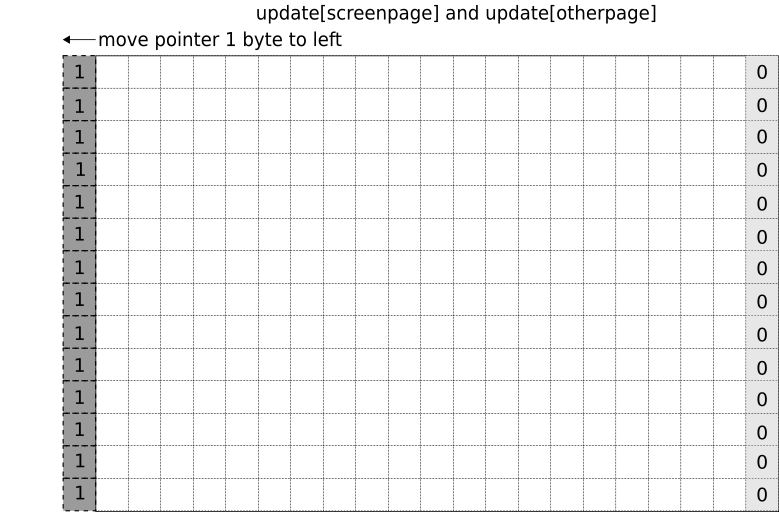
\includegraphics[width=.9\textwidth]{screenshots_300dpi/game/Scroll_KC4_6_1-scroll_update.png}
 \label{fig:kc4_6_update_array}  
\end{figure}
\end{minipage}

\begin{figure}[H]
\centering
 \fullimage{/game/Scroll_KC4_6_3.png}
 \caption{Step 2: Update sprites}
 \label{fig:kc4_6_add_column}
\end{figure}


\begin{minipage}{.4\textwidth}
These steps are the same as Commander Keen 1-3, meaning removal blocks will be marked with a '2' and copied from the master to the buffer screen and sprites are copied to the buffer screen and marked with a '3' in both tile arrays.
 \end{minipage}
\begin{minipage}{.6\textwidth}
\begin{figure}[H]
  \centering
 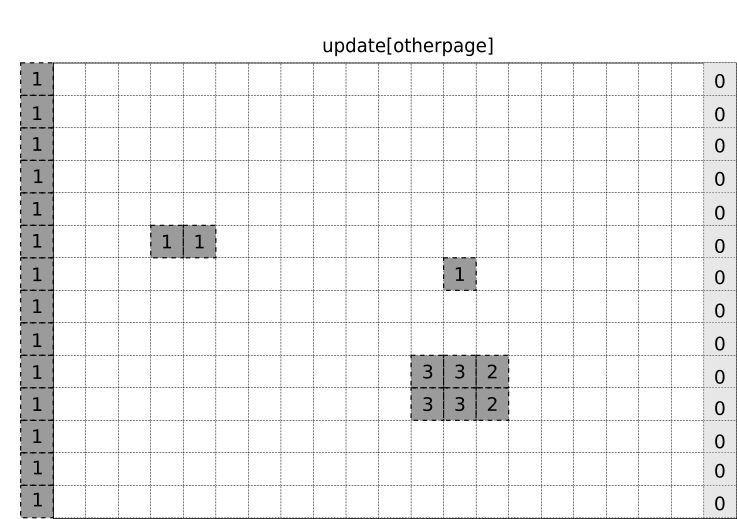
\includegraphics[width=.9\textwidth]{screenshots_300dpi/game/Scroll_KC4_6_1-scroll_update_sprite.png}
 \label{fig:kc4_6_update_array}  
\end{figure}
\end{minipage}

\pagebreak

\begin{figure}[H]
\centering
 \fullimage{/game/Scroll_KC4_6_final.png}
 \caption{Step 6: Swap buffer and screen page}
 \label{fig:k4_6_update_final}
\end{figure}


\begin{minipage}{.4\textwidth}
Swap the buffer and screen page by updating the CRTR start address and horizontal Pel Panning. The buffer tile array is cleared to '0', and then buffer and visible tile arrays are swapped. Then step 1 is repeated. 
 \end{minipage}
\begin{minipage}{.6\textwidth}
\begin{figure}[H]
  \centering
 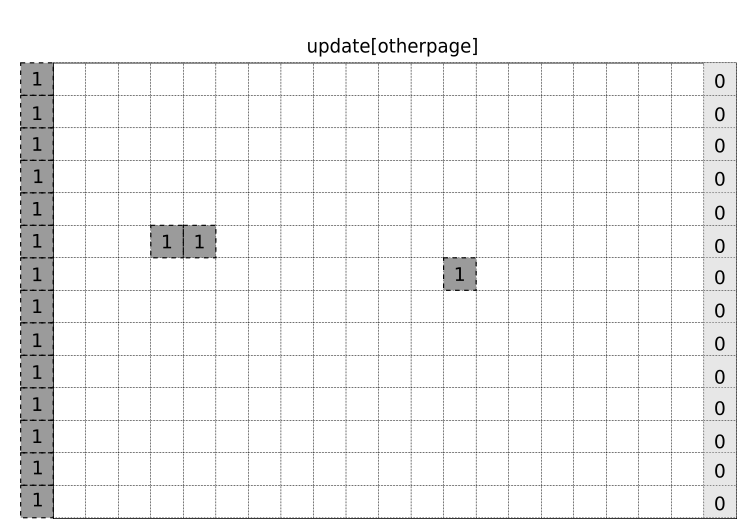
\includegraphics[width=.9\textwidth]{screenshots_300dpi/game/Scroll_KC4_6_1-scroll_update_final.png}
 \label{fig:kc4-6_update_final_img_1}  
\end{figure}
\end{minipage}

\pagebreak





\section{Refresh video screen}
Here explain with code. Focus on when to perform screen refresh (waiting for vertical retracement)

\section{A.I.}
To simulate enemies, some objects are allowed to "think" and take actions like firing, walking,
or emitting sounds. These thinking objects are called "actors".
Actors are programmed via a state machine. They can be aggressive, sneaky, or dumb
(XXX for instance). To model their behavior, all enemies have an associated state:

\section{Drawing Sprites}
Explain how animation are performed. Should we somehow also explain sprites on other systems, like Nintendo, etc.?\\
Once the state of the actor is updated, it is time to render the actor on the screen. This is a two step operation.
\begin{enumerate}
\item Update the state and move actors within the active region.
\item Determinate if a actor has changed or moved
\item Update the actor by removing and drawing sprites to it's new position
\end{enumerate}

\subsection{Visible actor determination}


\subsection{Clipping}
Before we draw a sprite on the screen, the engine determines if the boundaries of a sprite are hitting a wall or floor. This is called clipping and ensures an actor doesn't fall through a floor or walks through a vertical wall.\\
To define whether a tile is a wall or floor, a tile can be enriched with wall information. For each level map the tile info variable \cw{tinf} contains a \cw{NORTHWALL}, \cw{SOUTHWALL}, \cw{EASTWALL} and \cw{WESTWALL} map as illustrated in Fig \ref{fig:clip_tinf}.


\begin{figure}
\centering
\begin{subfigure}{.33\textwidth}
  \centering
  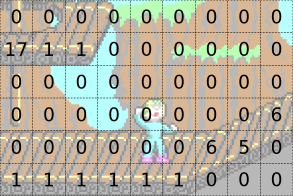
\includegraphics[width=.9\textwidth]{screenshots_300dpi/game/clip_tinf_1.png}
  \caption{Tile info map NORTHWALL}
  \label{fig:clip_tinf_n}
\end{subfigure}%
\begin{subfigure}{.33\textwidth}
  \centering
  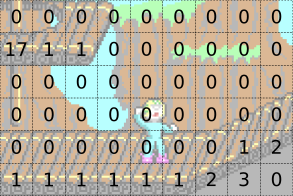
\includegraphics[width=.9\textwidth]{screenshots_300dpi/game/clip_tinf_south.png}
  \caption{Tile info map SOUTHWALL}
  \label{fig:clip_tinf_s}
\end{subfigure}
\begin{subfigure}{.33\textwidth}
  \centering
  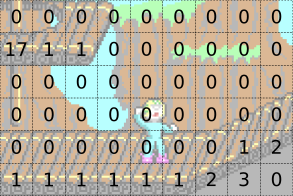
\includegraphics[width=.9\textwidth]{screenshots_300dpi/game/clip_tinf_south.png}
  \caption{Tile info map EASTWALL UPDATE!!!}
  \label{fig:clip_tinf_e}
\end{subfigure}
\caption{Tile clipping map}
\label{fig:clip_tinf}
\end{figure}

\par
When the sprite boundary is hitting a wall on the right (east), it will update the sprite movement to ensure the sprite right boundary is equal to the right side of the tile as illustrated in Fig. XX. The east/west wall clipping logic is covered by \cw{ClipToEastWalls (objtype *ob)} and \cw{ClipToWestWalls (objtype *ob)}. 
\\
\begin{minipage}{\textwidth}
  \lstinputlisting[language=C]{code/clip_east_wall.c}
\end{minipage}
\label{wallclip_array}
\par
The clipping for top and bottom is a bit more complex, as the engine also needs to take walking on slopes into account. After the sprite is clipped to the top or bottom of the wall tile, an offset can be applied to move a sprite up or down a slope. 
\\
\begin{minipage}{\textwidth}
  \lstinputlisting[basicstyle=\fontsize{8}{10}\selectfont]{code/wallclip_array.c}
\end{minipage}
\label{wallclip_array}
\par
When a sprite is clipped to a top or bottom tile, the corresponding midpoint pixels (0-15) and tile info map defines the offset from this top or bottom tile.
\begin{figure}[H]
  \centering
  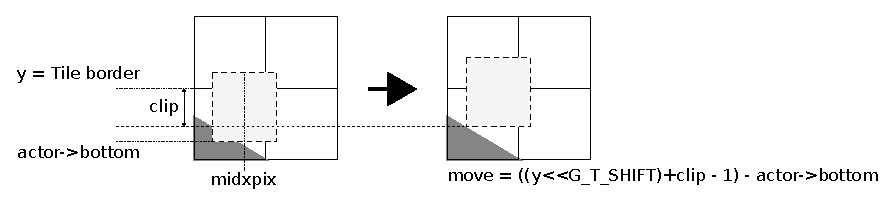
\includegraphics[width=\textwidth]{imgs/drawings/clipping.eps}
  \label{fig:clipping_north}
  \caption{Clipping NORTHWALL}
\end{figure}

\par
\begin{minipage}{\textwidth}
  \lstinputlisting[language=C]{code/clip_north_wall.c}
\end{minipage}
\label{wallclip_array}
\par



\end{document}